\documentclass[11pt,a4paper]{article}
\usepackage[margin=1in]{geometry}
\usepackage[T1]{fontenc}
\usepackage{lmodern}
\usepackage{microtype}
\usepackage{amsmath}
\usepackage{xcolor}
\definecolor{kthblue}{HTML}{004791}
\usepackage[hyphens,spaces,obeyspaces]{xurl}
\usepackage{booktabs}
\usepackage{tabularx}
\usepackage{array}
\usepackage{needspace}
\usepackage{float}
\usepackage{enumitem}
\usepackage{graphicx}
\usepackage{fancyhdr}
\usepackage{parskip}
\usepackage{hyperref}

\newcolumntype{Y}{>{\raggedright\arraybackslash}X}
\emergencystretch=2em
\setlength{\tabcolsep}{5pt}
\renewcommand{\arraystretch}{1.18}
\renewcommand{\contentsname}{}
\newcommand{\tocentry}[1]{\addcontentsline{toc}{section}{#1}}

\hypersetup{
    colorlinks=true,
    linkcolor=kthblue,
    urlcolor=kthblue,
    pdftitle={Scalable Machine Learning -- Lab 1, Role C Report},
    pdfauthor={Role C},
}
\title{Lab 1 -- Role C Report}
\author{Role C}
\date{24 November 2026}

\pagestyle{fancy}
\fancyhf{}
\fancyhead[L]{\small Scalable Machine Learning -- Role C}
\fancyhead[R]{\small Lab 1}
\fancyfoot[C]{\small \thepage}
\renewcommand{\headrulewidth}{0.4pt}
\setlength{\headheight}{14pt}

\begin{document}

\pagenumbering{gobble}
\hypersetup{pageanchor=false}
\begin{titlepage}
\thispagestyle{empty}
\centering
\vspace*{1.0cm}

\begingroup
\setlength{\fboxsep}{12pt}
\colorbox{kthblue}{
\includegraphics[height=2.8cm]{kth-logo.png}}
\endgroup

\vspace{0.35cm}
{\footnotesize KTH Electrical Engineering and Computer Science}

\vspace{1.6cm}

{\LARGE\bfseries Lab 1 -- Role C Report\\[0.45cm]
Augmentation Robustness, STL-10\\[0.25cm]
Generalization, and Cost Tradeoffs}

\vspace{1.2cm}

{\small Scalable Machine Learning}

\vfill

{\large Role C}

\vspace{1.4cm}

{\small Stockholm, 24 November 2026}
\vspace*{0.3cm}
\end{titlepage}
\hypersetup{pageanchor=true}
\pagenumbering{arabic}

\tableofcontents
\vspace{1.5em}

\section*{Introduction}
\tocentry{Introduction}

This report covers the Role C part of Lab 1: Task 4 (data augmentation and
robustness to fixed corruptions), Challenge 2 (cross-domain generalization
from CIFAR-10 to STL-10), and Task 6 (cost and tradeoff benchmarking). Every
number comes from five completed 30-epoch training runs and a frozen
evaluation protocol, with measurements stored in the result JSON files and
CSV summaries in \texttt{lab1/results/}; the executed notebook with all
outputs is linked in the reproduction section.

\section*{Experimental protocol}
\tocentry{Experimental protocol}

CIFAR-10 is split into 45,000 training and 5,000 validation images with a
fixed split, and the 10,000 test images are reserved for final evaluation.
Every run trains for 30 epochs with batch size 128, which gives 1,350,000
trained samples per run, using SGD with momentum 0.9, weight decay $5\times10^{-4}$,
a cosine learning rate schedule, and FP32 precision. AlexNet trains with
learning rate 0.01 and ResNet-18 with 0.1. The checkpoint with the best
validation accuracy is kept for all later evaluation.

The frozen experiment matrix has five configurations
(Table~\ref{tab:matrix}).

\begin{table}[H]
\centering
\small
\begin{tabularx}{\textwidth}{@{}Y l r l@{}}
\toprule
\textbf{exp\_id} & \textbf{model} & \textbf{seed} & \textbf{augmentation} \\
\midrule
\texttt{t6\_alexnet\_cifar\_no\_aug\_s42} & alexnet\_cifar & 42 & none \\
\texttt{t4\_resnet18\_cifar\_no\_aug\_s42} & resnet18\_cifar & 42 & none \\
\texttt{t4\_resnet18\_cifar\_crop\_flip\_s42} & resnet18\_cifar & 42 & crop32\_pad4\_hflip05 \\
\texttt{t6\_resnet18\_cifar\_crop\_flip\_s0} & resnet18\_cifar & 0 & crop32\_pad4\_hflip05 \\
\texttt{t6\_resnet18\_cifar\_crop\_flip\_s123} & resnet18\_cifar & 123 & crop32\_pad4\_hflip05 \\
\bottomrule
\end{tabularx}
\caption{Frozen experiment matrix: five configurations, one fixed split,
30 epochs each.}
\label{tab:matrix}
\end{table}

The corruption protocol is frozen in
\texttt{lab1/configs/corruptions\_t4.json} (version 1, seed 2223) and applied
to the same 10,000 test image IDs for every model. Each image gets an
independent generator seeded with $2223 + \texttt{image\_id}$, so a given
image receives pixel-identical corruption across models, DataLoader worker
counts, and evaluation sessions. The three conditions are rotation by a
uniformly sampled angle in $[-15, +15]$ degrees (bilinear resampling, fill
0), translation by independent integer offsets in $[-3, +3]$ pixels on each
axis (fill 0), and additive Gaussian noise with standard deviation 0.05,
clamped to $[0, 1]$. Clean and corrupted evaluations iterate over the same
IDs in the same order, which allows per-image pairing of predictions. All
five result files record the same SHA256 hash for the corruption config.

Model and augmentation choices were frozen before any test or STL-10
evaluation, and no augmentation search was performed; that is a deliberate
validation boundary, so crop plus flip is one reasonable choice rather than
a tuned optimum. STL-10 was used only for forward evaluation after freezing
and never influenced any selection.

Training ran on Google Colab Tesla T4 GPUs in FP32. All test, corruption,
and STL-10 evaluations ran on the Jade cluster node with an NVIDIA RTX 2000
Ada Generation GPU in FP32. The separate inference benchmark on that GPU
used 10 warmup runs, 50 measured runs, CUDA synchronization around each
timed region, and batch sizes 1 and 128. Training times below are T4 numbers
and inference times are Jade numbers; the two groups are reported separately
and never ranked against each other.

% =====================================================================
\clearpage
\section*{Task 4: augmentation and fixed-corruption robustness}
\tocentry{Task 4: augmentation and fixed-corruption robustness}

The augmented condition applies a random crop of size 32 with padding 4,
followed by a horizontal flip with probability $0.5$, to training images
only. Both transformations preserve CIFAR-10 labels in the usual sense: a 4-pixel padded crop
introduces small translations, and a horizontal flip does not change the
object category. This argument has limits, since a strong random crop can
cut off the object, so paired same-ID examples are kept for qualitative
checks below.

\begin{table}[H]
\centering
\small
\begin{tabular}{@{}lrrr@{}}
\toprule
\textbf{condition} & \textbf{no-aug} & \textbf{crop+flip} & \textbf{difference} \\
\midrule
clean & 0.8658 & 0.9308 & $+0.0650$ \\
rotation 15 deg & 0.7680 & 0.8871 & $+0.1191$ \\
translation 3 px & 0.8014 & 0.9281 & $+0.1267$ \\
Gaussian noise (std 0.05) & 0.7133 & 0.6814 & $-0.0319$ \\
mean of three corruptions & 0.7609 & 0.8322 & $+0.0713$ \\
\bottomrule
\end{tabular}
\caption{Seed-42 ResNet results on the shared 10,000 test IDs.}
\label{tab:t4-acc}
\end{table}

Accuracy drop is the same model's clean accuracy minus its corrupted
accuracy. Prediction flip rate uses all 10,000 IDs as the denominator;
clean-correct-to-wrong rate instead uses that model's own clean-correct
predictions.

\begin{table}[H]
\centering
\footnotesize
\setlength{\tabcolsep}{3pt}
\begin{tabular}{@{}llrrrr@{}}
\toprule
\textbf{condition} & \textbf{model} & \textbf{acc.\ drop} & \textbf{pred.\ flip rate} & \textbf{correct$\to$wrong} & \textbf{rate} \\
\midrule
rotation & no-aug & 0.0978 & 0.1892 & 1270 & 0.1467 \\
rotation & crop+flip & 0.0437 & 0.0878 & 593 & 0.0637 \\
translation & no-aug & 0.0644 & 0.1715 & 1032 & 0.1192 \\
translation & crop+flip & 0.0027 & 0.0373 & 173 & 0.0186 \\
noise & no-aug & 0.1525 & 0.2460 & 1767 & 0.2041 \\
noise & crop+flip & 0.2494 & 0.3106 & 2658 & 0.2856 \\
\bottomrule
\end{tabular}
\caption{Per-image pairing against each model's own clean predictions.}
\label{tab:t4-paired}
\end{table}

Crop plus flip improves clean accuracy by 6.5 points and both geometric
corruptions; translation is almost saturated for the augmented model (drop
0.0027). Gaussian noise is the exception: augmented noise accuracy is
0.6814, which is 0.0319 below the no-augmentation model's 0.7133. Relative
to its own clean accuracy, the augmented model drops from 0.9308 to 0.6814
(drop 0.2494). It turns 2,658 of its 9,308 clean-correct predictions wrong
(0.2856), versus 1,767 of 8,658 for the no-augmentation model (0.2041).
Across all five configurations, noise is the weakest condition for all four
ResNets, while the AlexNet baseline is weakest under rotation (0.6829) and
reaches the highest noise accuracy of any run (0.7756). Crop plus flip
improves clean and geometric robustness and hurts noise robustness in this
setup, so a general robustness gain cannot be claimed.

Final train\_eval accuracy, measured by a deterministic, unaugmented pass
over the 45,000 training IDs and distinct from running augmented
train\_acc, is 0.9972 for the augmented ResNet and 1.0 for the
no-augmentation ResNet. Both models therefore fit the training data closely,
so training fit alone does not explain the augmented model's worse noise
accuracy. Under noise the augmented model's per-class accuracy is lowest on
dog (0.422), airplane (0.474), and cat (0.543), while frog stays at 0.966.
One possible reading is that the noise destroys fine texture while frog
predictions rely more on color or coarse shape, but this attribution would
need a controlled experiment before it can be stated as a cause.

The augmentation is nearly free at training time. On the T4, the augmented
ResNet trained in 1,859.8\,s versus 1,855.4\,s without augmentation
($+4.5$\,s, about $+0.24\%$; 62.0\,s versus 61.8\,s per epoch on average),
with identical peak memory of 803\,MB. On Jade, one pass over the 10,000
test images took 1.418 to 1.435\,s for every ResNet condition, with
per-model differences between corrupted and clean runs below 0.01\,s;
AlexNet took 0.448 to 0.635\,s. These timings include DataLoader work and
CPU-side corruption, so they bound the end-to-end evaluation overhead and
say nothing about the pure transform cost.

The frozen corruptions are mild by design. Stronger rotation, heavier
cropping, or stronger noise could make the correct label ambiguous even for
a human annotator, which would confound robustness measurement with label
noise; this is one reason the paired same-ID examples below are reported
next to the aggregate numbers.

\begin{figure}[H]
\centering
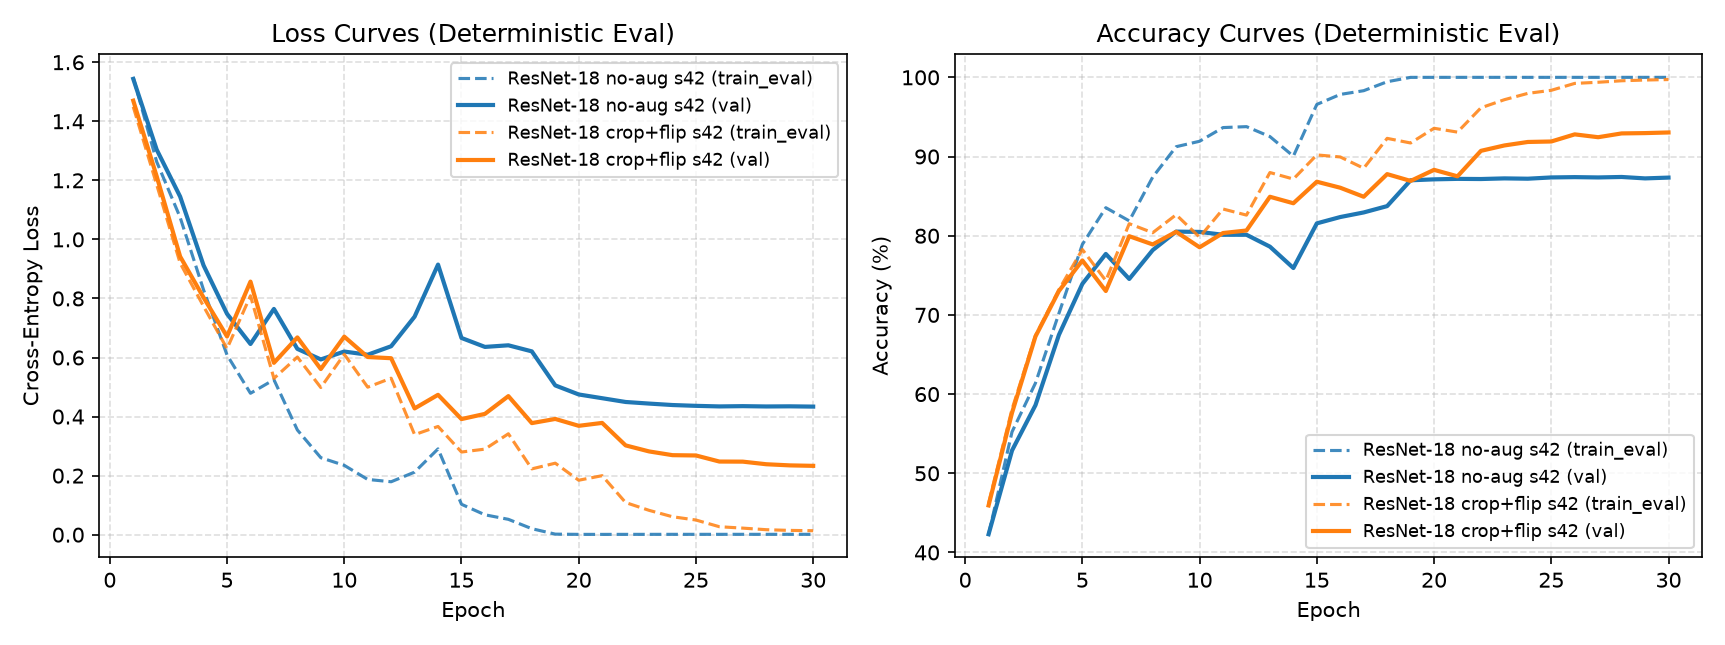
\includegraphics[width=0.9\textwidth]{../results/figures/t4_learning_curves.png}
\caption{Validation and training curves over 30 epochs for the seed-42
ResNet pair. The augmented run trails early and finishes higher.}
\label{fig:t4-curves}
\end{figure}

\begin{figure}[H]
\centering
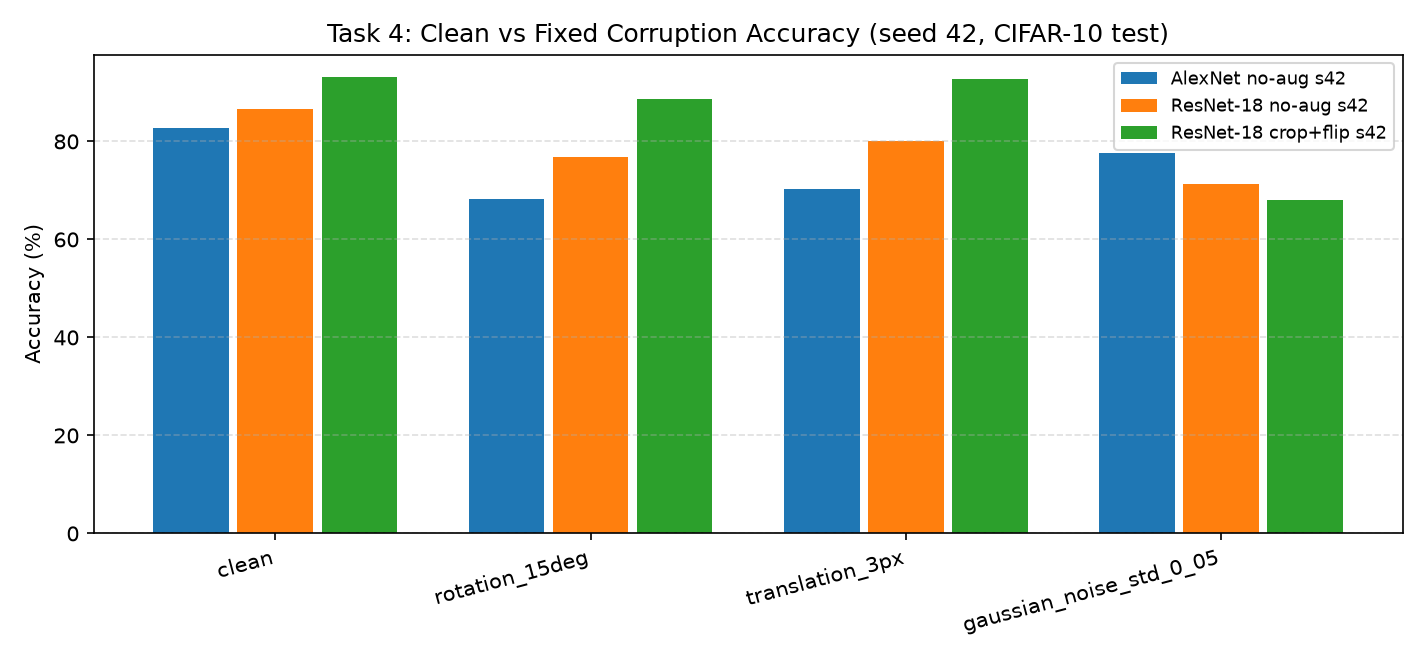
\includegraphics[width=0.9\textwidth]{../results/figures/t4_corruption_accuracy.png}
\caption{Accuracy of the three seed-42 configurations on clean CIFAR-10 test
and the three frozen corruptions. Crop plus flip helps on clean, rotation,
and translation but not on Gaussian noise.}
\label{fig:t4-corruption-acc}
\end{figure}

\begin{figure}[H]
\centering
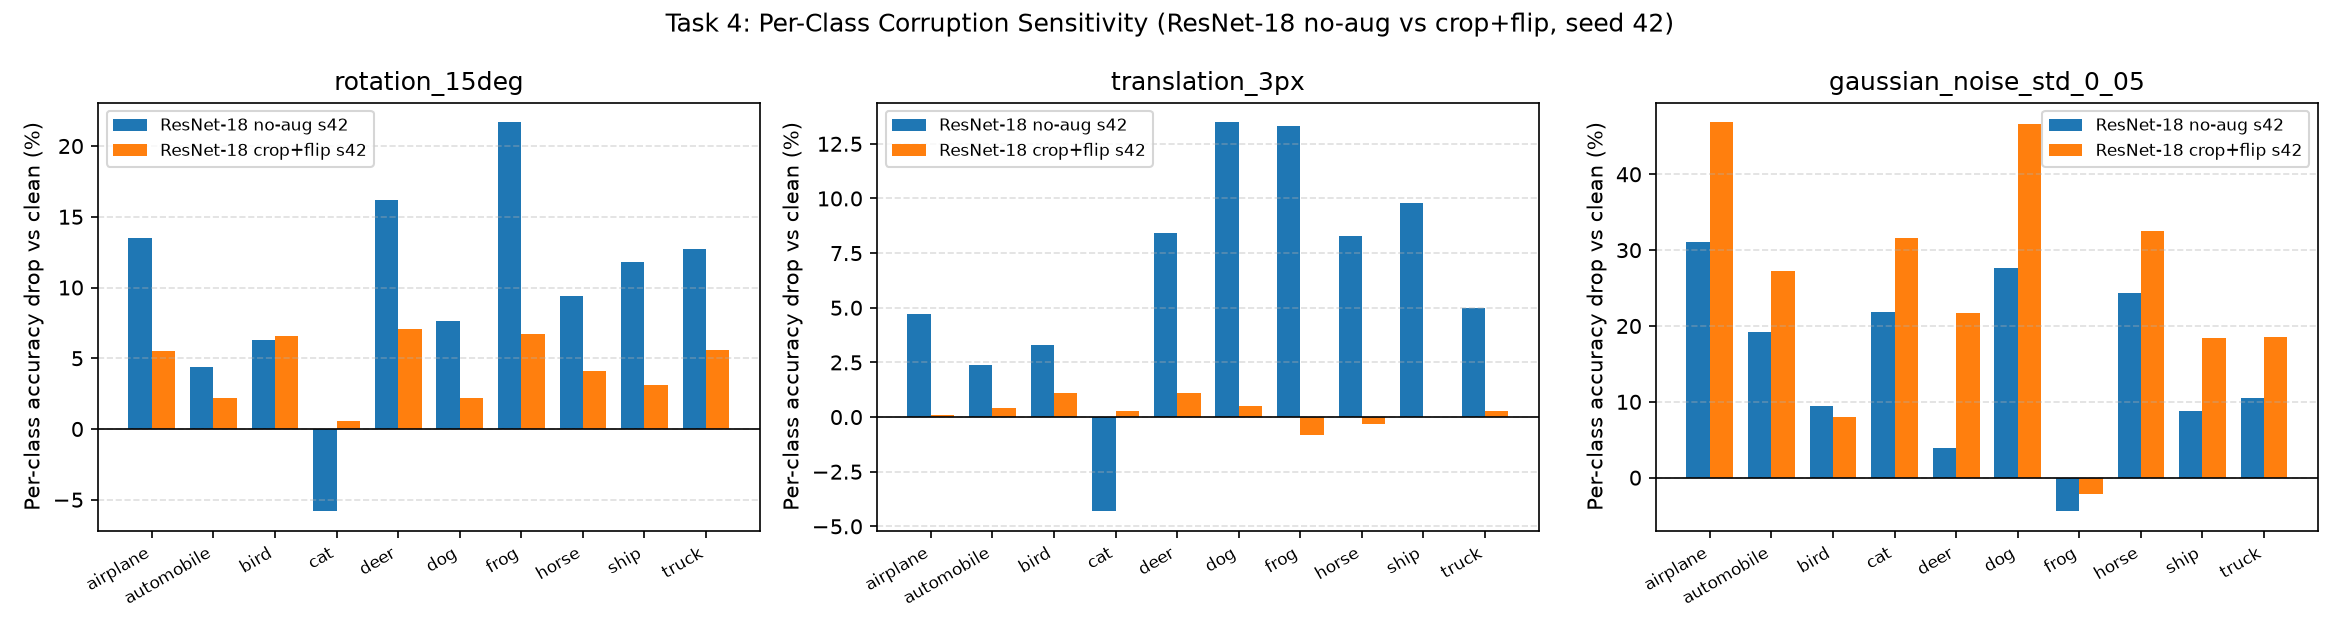
\includegraphics[width=0.9\textwidth]{../results/figures/t4_per_class_drops.png}
\caption{Per-class accuracy drops from clean to each corruption for the
seed-42 ResNet pair, showing where the augmented model gains and where it
loses.}
\label{fig:t4-per-class}
\end{figure}

\begin{figure}[H]
\centering
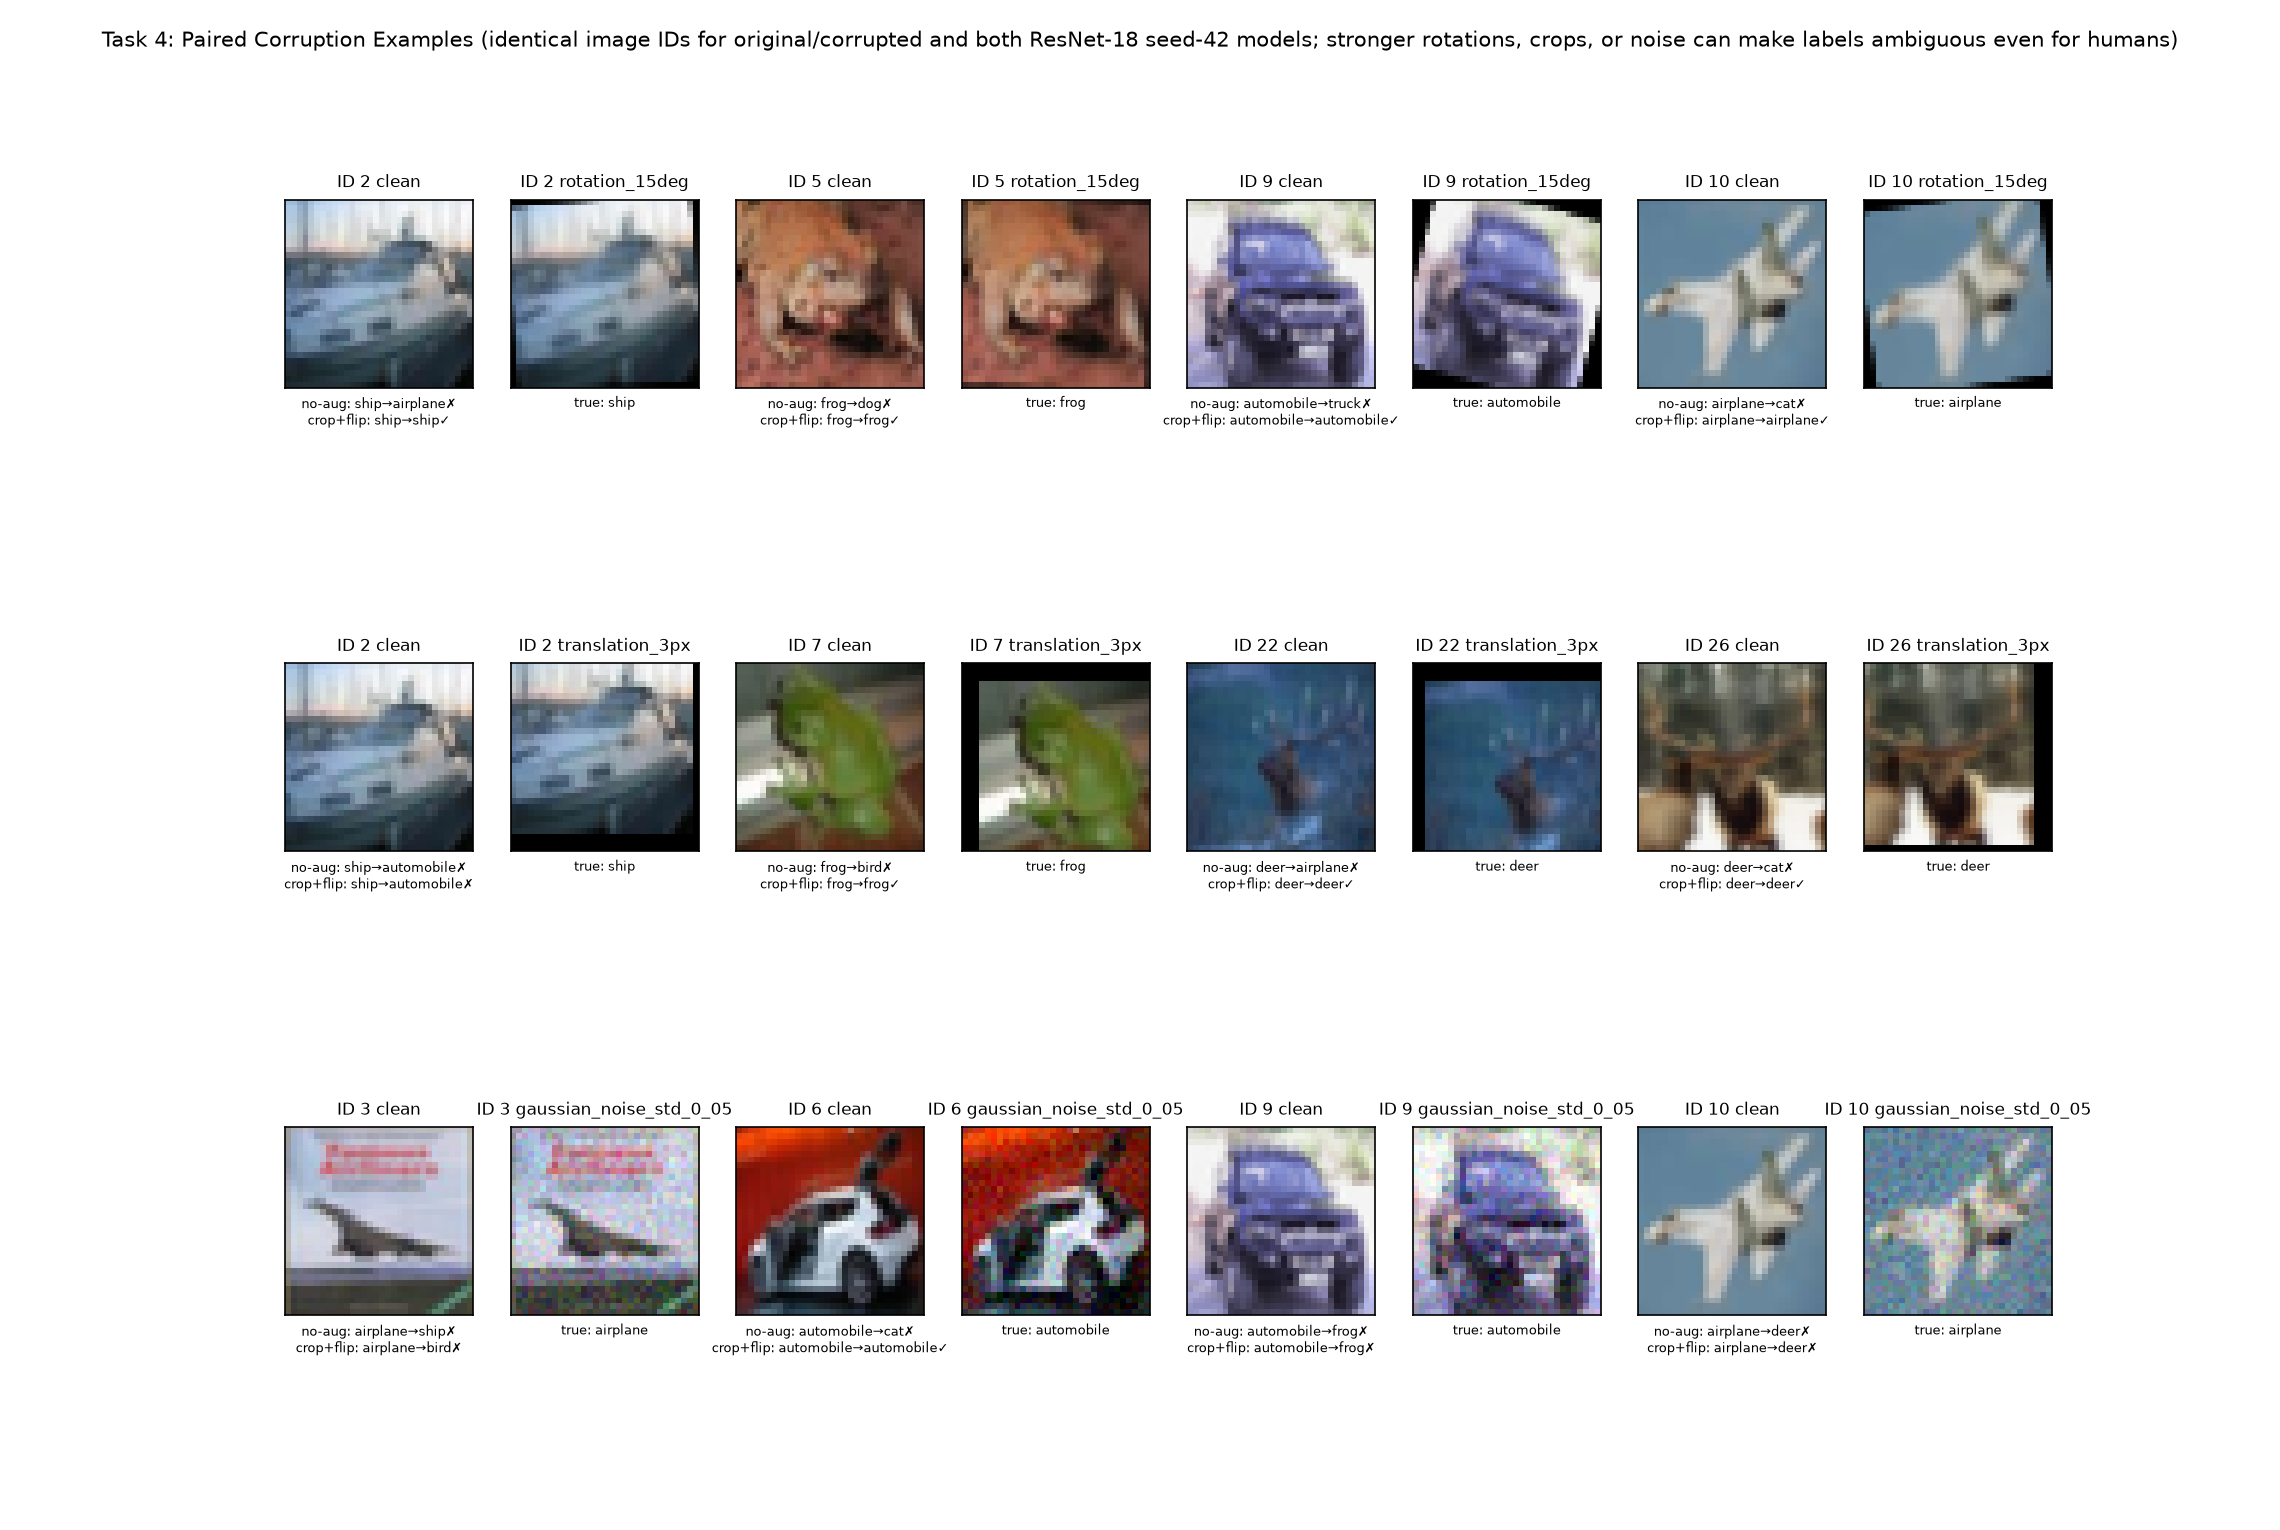
\includegraphics[width=\textwidth]{../results/figures/t4_corruption_examples.png}
\caption{Paired same-ID corruption examples for cases the no-augmentation
ResNet classifies correctly when clean and incorrectly when corrupted, with
both models' predictions shown on identical images.}
\label{fig:t4-examples}
\end{figure}

% =====================================================================
\clearpage
\section*{Challenge 2: CIFAR-10 to STL-10 generalization}
\tocentry{Challenge 2: CIFAR-10 to STL-10 generalization}

STL-10 test contains 8,000 images at $96\times96$ pixels over ten classes,
including monkey, which has no CIFAR-10 counterpart. Filtering out monkey
leaves 7,200 images over the nine shared classes (airplane, bird,
automobile, cat, deer, dog, horse, ship, truck), whose STL labels are mapped
onto CIFAR indices. Images are resized from $96\times96$ to $32\times32$
with bilinear interpolation and antialiasing, then normalized with CIFAR-10
training statistics before the forward pass. Two scoring conventions are
reported: 10-way accuracy without logit masking, which also yields the frog
leakage rate (the fraction of STL images predicted as frog, a class STL does
not contain), and 9-way masked accuracy, the argmax restricted to the nine
shared logits. The CIFAR reference is the 9-way masked accuracy over the
9,000 shared-class test images, and the domain drop is defined as
$\texttt{cifar10\_test\_9way\_acc} - \texttt{stl10\_9way\_masked\_acc}$.

\begin{table}[H]
\centering
\footnotesize
\setlength{\tabcolsep}{4pt}
\begin{tabular}{@{}lrrrrrr@{}}
\toprule
\textbf{model (seed 42)} & \textbf{CIFAR 9-way} & \textbf{STL 10-way} & \textbf{frog leak} & \textbf{STL 9-way} & \textbf{macro F1} & \textbf{domain drop} \\
\midrule
alexnet no-aug & 0.8310 & 0.6675 & 0.0314 & 0.6825 & 0.6790 & 0.1485 \\
resnet no-aug & 0.8683 & 0.7107 & 0.0351 & 0.7267 & 0.7221 & 0.1417 \\
resnet crop+flip & 0.9339 & 0.8014 & 0.0185 & 0.8108 & 0.8088 & 0.1231 \\
\bottomrule
\end{tabular}
\caption{Cross-domain results for the three seed-42 models. ``frog leak''
is the frog leakage rate and ``STL 9-way'' the masked 9-way accuracy.}
\label{tab:challenge2}
\end{table}

The augmented ResNet has both the highest absolute STL accuracy and the
smallest drop (0.1231 versus 0.1417 and 0.1485), and the lowest frog leakage
at 1.85\%. Its STL gain over the no-augmentation ResNet ($+0.0841$) is
larger than its CIFAR 9-way gain ($+0.0656$), which is consistent with crop
plus flip teaching geometric invariances that transfer across domains. With
one seed for the direct ResNet comparison, this correlation does not by
itself demonstrate a cause.

Per-class, the augmented ResNet's largest domain drops are dog (0.890 on
CIFAR, 0.589 on STL, drop 0.3013), cat (0.873 to 0.661, drop 0.2118), and
horse (0.942 to 0.791, drop 0.1507); the smallest are ship (0.0395) and deer
(0.0420). The no-augmentation ResNet also peaks on dog (0.3488) and
additionally on truck (0.2015), and AlexNet peaks on dog (0.3108), truck
(0.2788), and horse (0.1733). All three models share the dog weakness. A
plausible explanation is that resizing from $96\times96$ to $32\times32$
removes fine texture that STL's higher-resolution images carry, while the
models only ever saw the $32\times32$ CIFAR distribution. The per-class
numbers and the failure examples are consistent with this reading, but the
experiment does not isolate it, so it stays a hypothesis.

The failure figure samples up to six STL IDs from the deterministic union of
the three models' error sets and shows the same image next to all three
predictions. Pairing by ID keeps the comparison fair, and the union
construction means not every shown sample is misclassified by all three
models. STL-10 remained excluded from model, augmentation, and seed
selection and from the Task 6 recommendation.

\begin{figure}[H]
\centering
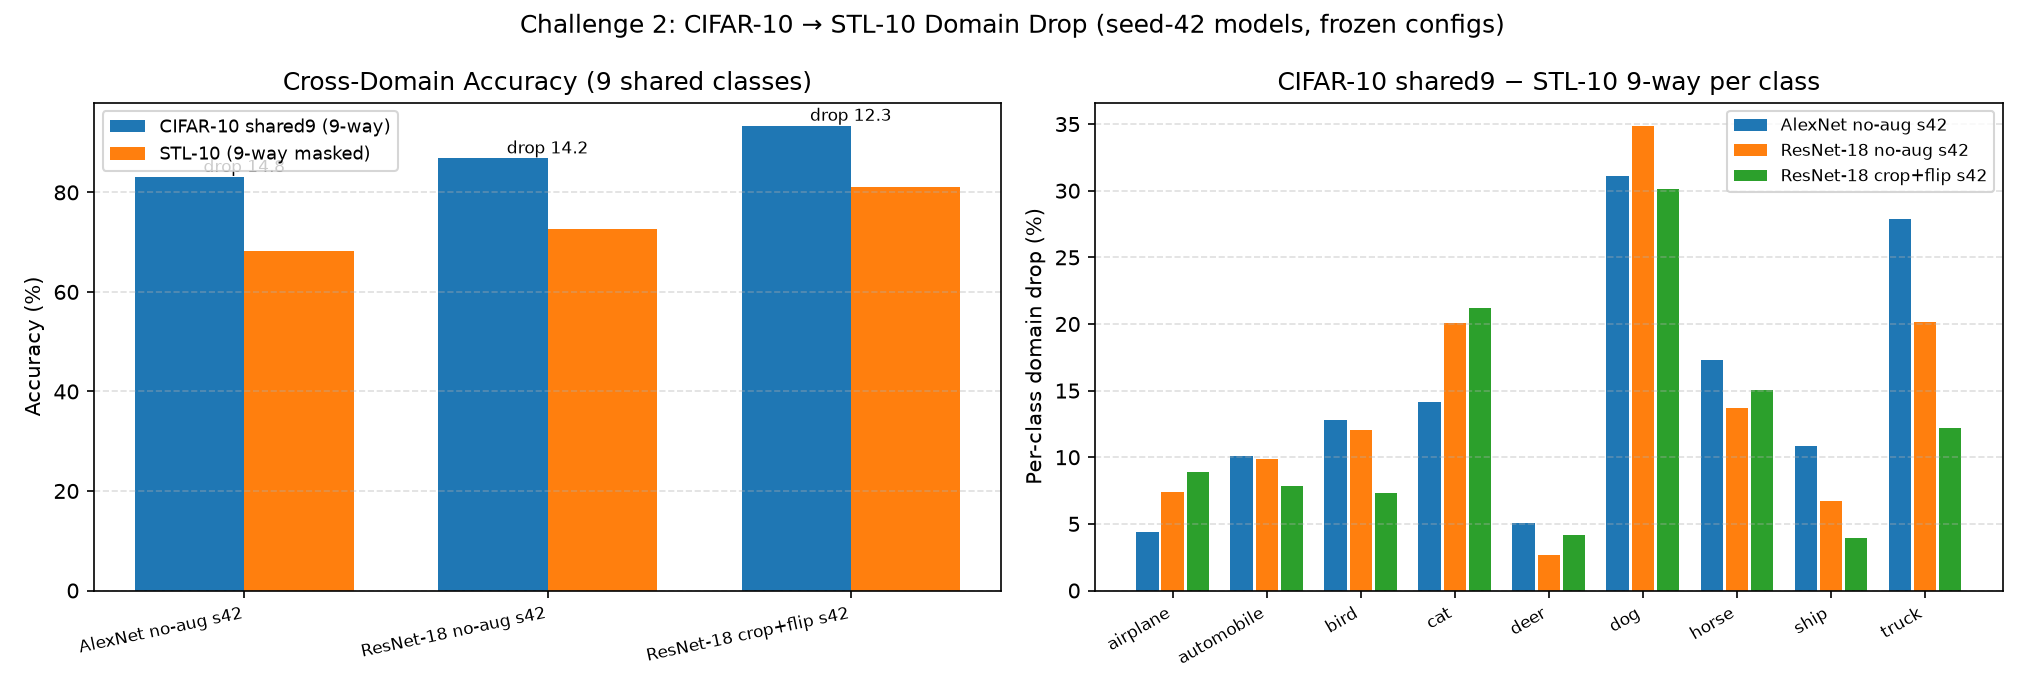
\includegraphics[width=0.95\textwidth]{../results/figures/challenge2_domain_drop.png}
\caption{CIFAR-10 shared 9-way versus STL-10 masked 9-way accuracy, total
and per-class domain drops for the three seed-42 models.}
\label{fig:c2-domain-drop}
\end{figure}

\begin{figure}[H]
\centering
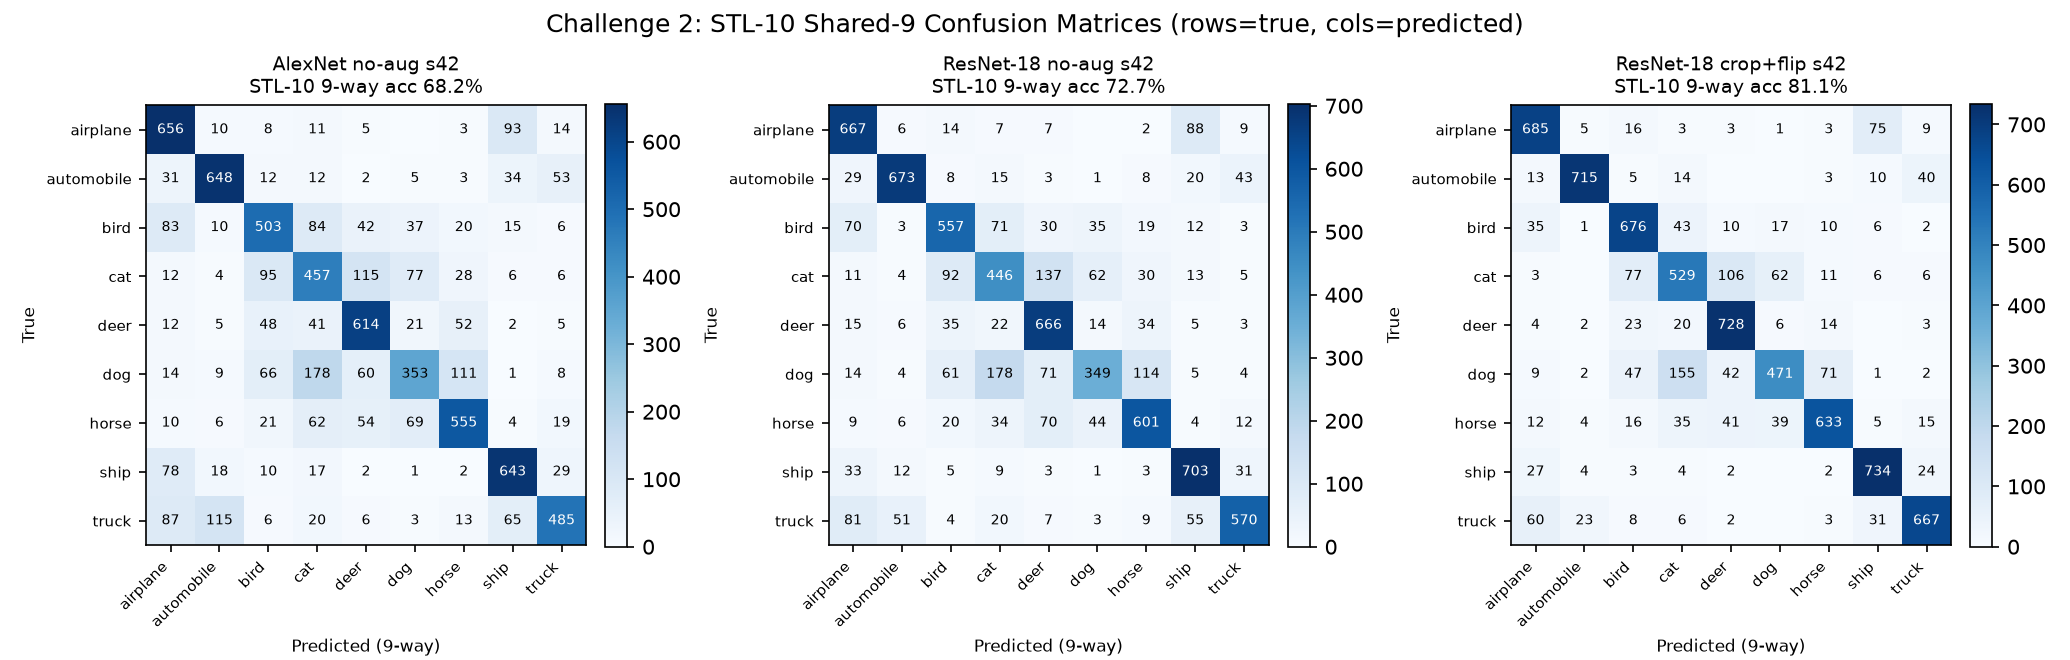
\includegraphics[width=0.95\textwidth]{../results/figures/challenge2_stl10_confusion.png}
\caption{Shared 9-class confusion matrices on STL-10 for the three seed-42
models.}
\label{fig:c2-confusion}
\end{figure}

\begin{figure}[H]
\centering
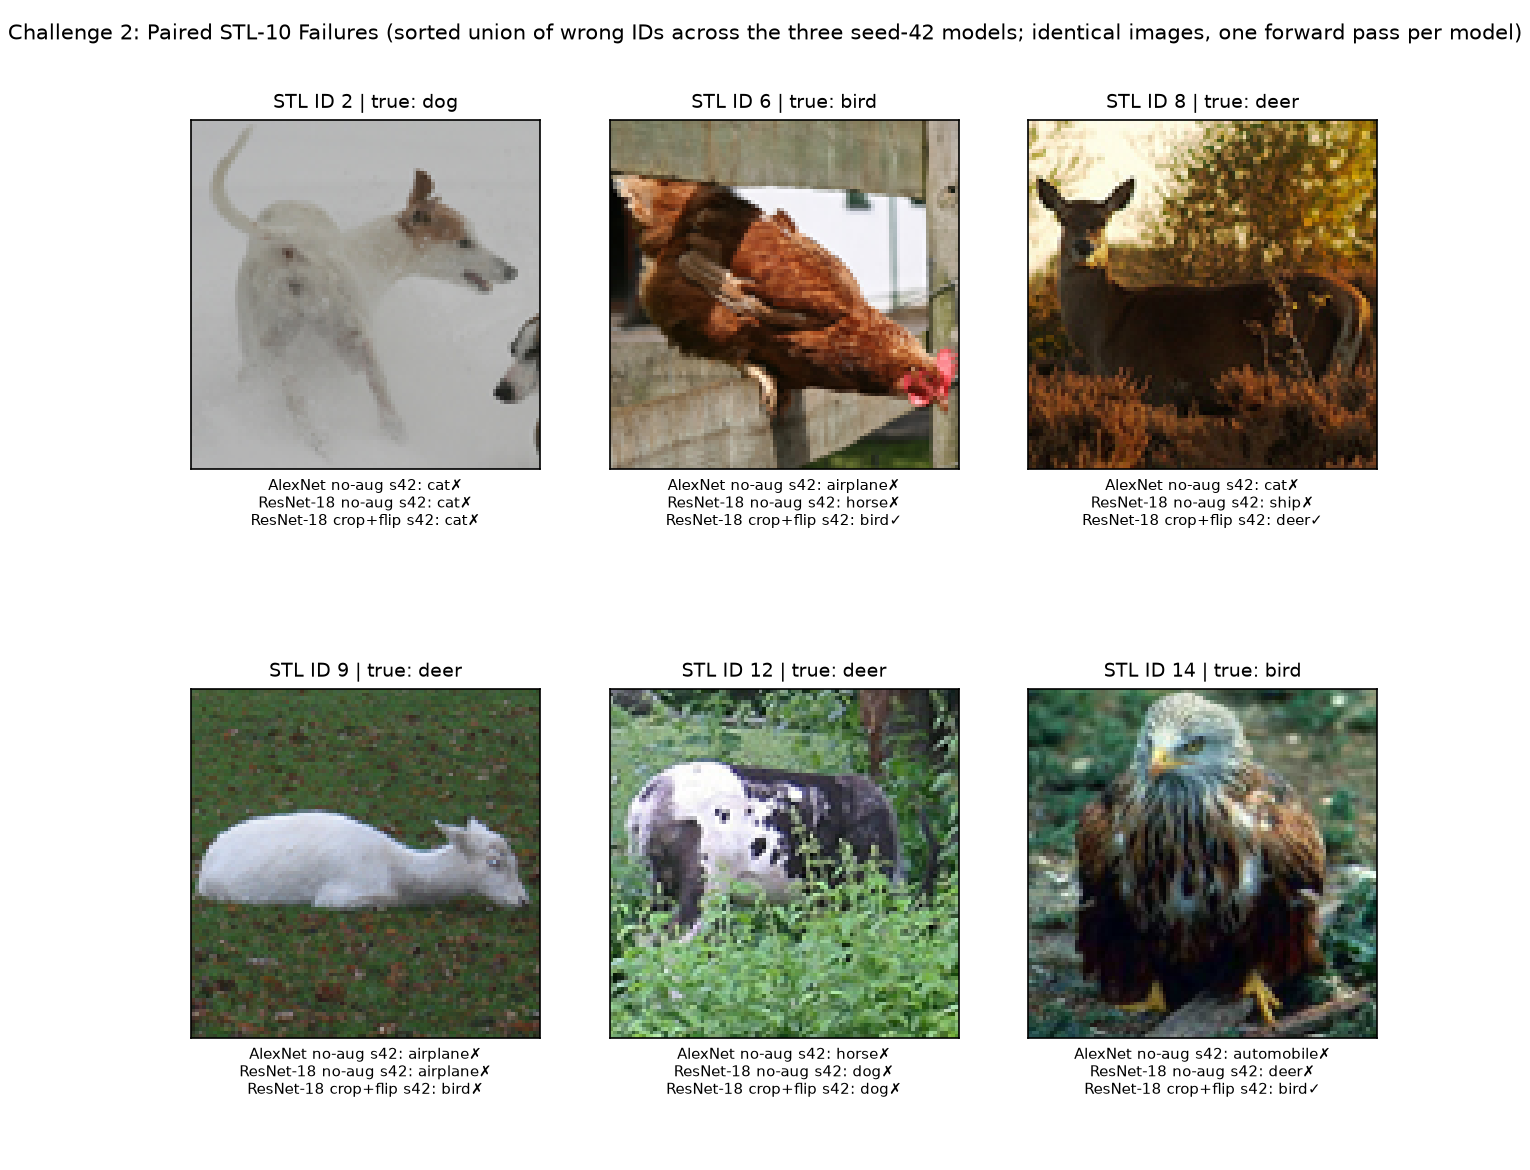
\includegraphics[width=\textwidth]{../results/figures/challenge2_stl10_failures.png}
\caption{Paired STL-10 failure examples drawn from the deterministic union
of the three models' error IDs. Each image is shown with all three
predictions; not every sample is wrong under all three models.}
\label{fig:c2-failures}
\end{figure}

% =====================================================================
\clearpage
\section*{Task 6: cost and tradeoffs}
\tocentry{Task 6: cost and tradeoffs}

Tables~\ref{tab:t6-cost} and~\ref{tab:t6-inference} collect costs and
accuracy for all five configurations. Training columns are measured on the
Tesla T4 and inference columns on the Jade RTX 2000 Ada; the two hardware
groups are never mixed in one comparison.

\begin{table}[H]
\centering
\footnotesize
\setlength{\tabcolsep}{4pt}
\begin{tabular}{@{}lrrrrr@{}}
\toprule
\textbf{configuration} & \textbf{params} & \textbf{T4 train (s)} & \textbf{T4 peak mem (MB)} & \textbf{clean} & \textbf{mean corr.} \\
\midrule
alexnet no-aug s42 & 6.98M & 353.7 & 316.9 & 0.8266 & 0.7207 \\
resnet no-aug s42 & 11.17M & 1,855.4 & 803.0 & 0.8658 & 0.7609 \\
resnet crop+flip s42 & 11.17M & 1,859.8 & 803.0 & 0.9308 & 0.8322 \\
resnet crop+flip s0 & 11.17M & 1,858.5 & 803.0 & 0.9279 & 0.8253 \\
resnet crop+flip s123 & 11.17M & 1,856.0 & 803.0 & 0.9292 & 0.8221 \\
\bottomrule
\end{tabular}
\caption{Parameter counts, Tesla T4 training costs, and CIFAR accuracy for
all five configurations.}
\label{tab:t6-cost}
\end{table}

\begin{table}[H]
\centering
\small
\begin{tabular}{@{}lrrr@{}}
\toprule
\textbf{configuration} & \textbf{Jade bs=1 (ms)} & \textbf{Jade bs=128 (ms/batch)} & \textbf{Jade throughput (img/s)} \\
\midrule
alexnet no-aug s42 & 0.309 & 4.50 & 28,467 \\
resnet no-aug s42 & 0.906 & 16.80 & 7,621 \\
resnet crop+flip s42 & 0.914 & 16.86 & 7,593 \\
resnet crop+flip s0 & 0.852 & 16.90 & 7,575 \\
resnet crop+flip s123 & 0.849 & 16.89 & 7,577 \\
\bottomrule
\end{tabular}
\caption{FP32 inference performance on the Jade RTX 2000 Ada GPU.}
\label{tab:t6-inference}
\end{table}

Judged only on CIFAR test accuracy, the fixed corruption suite, and compute
cost, the crop-plus-flip ResNet-18 family gives the strongest accuracy-cost
balance. Across seeds 42, 0, and 123 its mean clean accuracy is 0.9293 and
its mean corrupted accuracy is 0.8265 (range 0.8221--0.8322); every seed is
highest on both metrics among these five configurations. Seed 42 still has
the single highest clean and mean-corrupted values, but one seed cannot
establish that it is a better seed choice than 0 or 123. Augmentation adds
about $0.24\%$ training time and no extra memory over the no-augmentation
ResNet, and its 0.914\,ms batch-1 latency stays within the same-device
comparison group. If latency or throughput dominates the deployment budget,
the AlexNet baseline is the alternative: 0.309\,ms batch-1 latency (about
one third of the ResNet), 28,467 images/s at batch 128 (about 3.7 times the
ResNet), and 354\,s of training, at the price of roughly 10.4 points of
clean accuracy and 11.2 points of mean corrupted accuracy. STL-10 results
played no role in this choice.

\begin{table}[H]
\centering
\small
\begin{tabular}{@{}lrrrr@{}}
\toprule
\textbf{metric} & \textbf{mean} & \textbf{sample std} & \textbf{min} & \textbf{max} \\
\midrule
best val acc & 0.9314 & 0.0019 & 0.9302 & 0.9336 \\
clean test acc & 0.9293 & 0.0015 & 0.9279 & 0.9308 \\
rotation acc & 0.8823 & 0.0042 & 0.8795 & 0.8871 \\
translation acc & 0.9261 & 0.0017 & 0.9250 & 0.9281 \\
noise acc & 0.6712 & 0.0100 & 0.6615 & 0.6814 \\
mean corrupted acc & 0.8265 & 0.0052 & 0.8221 & 0.8322 \\
STL 9-way masked & 0.8110 & 0.0017 & 0.8093 & 0.8128 \\
domain drop & 0.1202 & 0.0040 & 0.1156 & 0.1231 \\
train time (s) & 1858.1 & 1.93 & 1856.0 & 1859.8 \\
\bottomrule
\end{tabular}
\caption{Seed sensitivity over seeds 0, 42, and 123 for the augmented
ResNet.}
\label{tab:t6-seeds}
\end{table}

Clean and geometric metrics vary little across seeds (sample standard
deviation at most 0.0042). Noise varies most (sample standard deviation
0.0100, range 0.0199), and no seed is uniformly best: seed 42 has the
highest clean, mean-corrupted, rotation, and translation values, while seed
0 has the highest noise accuracy. These single-policy seed measurements
support the family-level recommendation but cannot establish an optimal
seed.

Validation accuracy at epochs 10, 20, and 30 against cumulative T4 time
shows how duration changes the picture. AlexNet reaches 0.8046, 0.8236, and
0.8294 at 112, 233, and 354\,s, about one fifth of the ResNet training cost,
but ends below both ResNet configurations. The no-augmentation ResNet
reaches 0.8048, 0.8712, and 0.8734 at 620, 1,238, and 1,855\,s and saturates
after epoch 20. The augmented ResNet (seed 42) reaches 0.7854, 0.8832, and
0.9304 at 622, 1,241, and 1,860\,s: it trails the no-augmentation run at
epoch 10 and overtakes it later, so the augmentation benefit depends on the
full schedule and is not worth its cost under a short training budget. Seeds
0 and 123 show the same shape, ending at 0.9302 and 0.9318.

For hardware sensitivity, Role A trained the same two architectures on an
NVIDIA GeForce RTX 5070 Ti Laptop GPU. The T4-to-RTX training time ratio is
about 1.42 for AlexNet (353.7\,s versus 248.2\,s) and 2.71 for ResNet
(1,855.4\,s versus 685.0\,s), while clean accuracy agrees within about 0.005
across the two setups. The two sides used different benchmark machines and
sessions, so these rows describe observed hardware sensitivity only and form
no same-device ranking.

\begin{figure}[H]
\centering
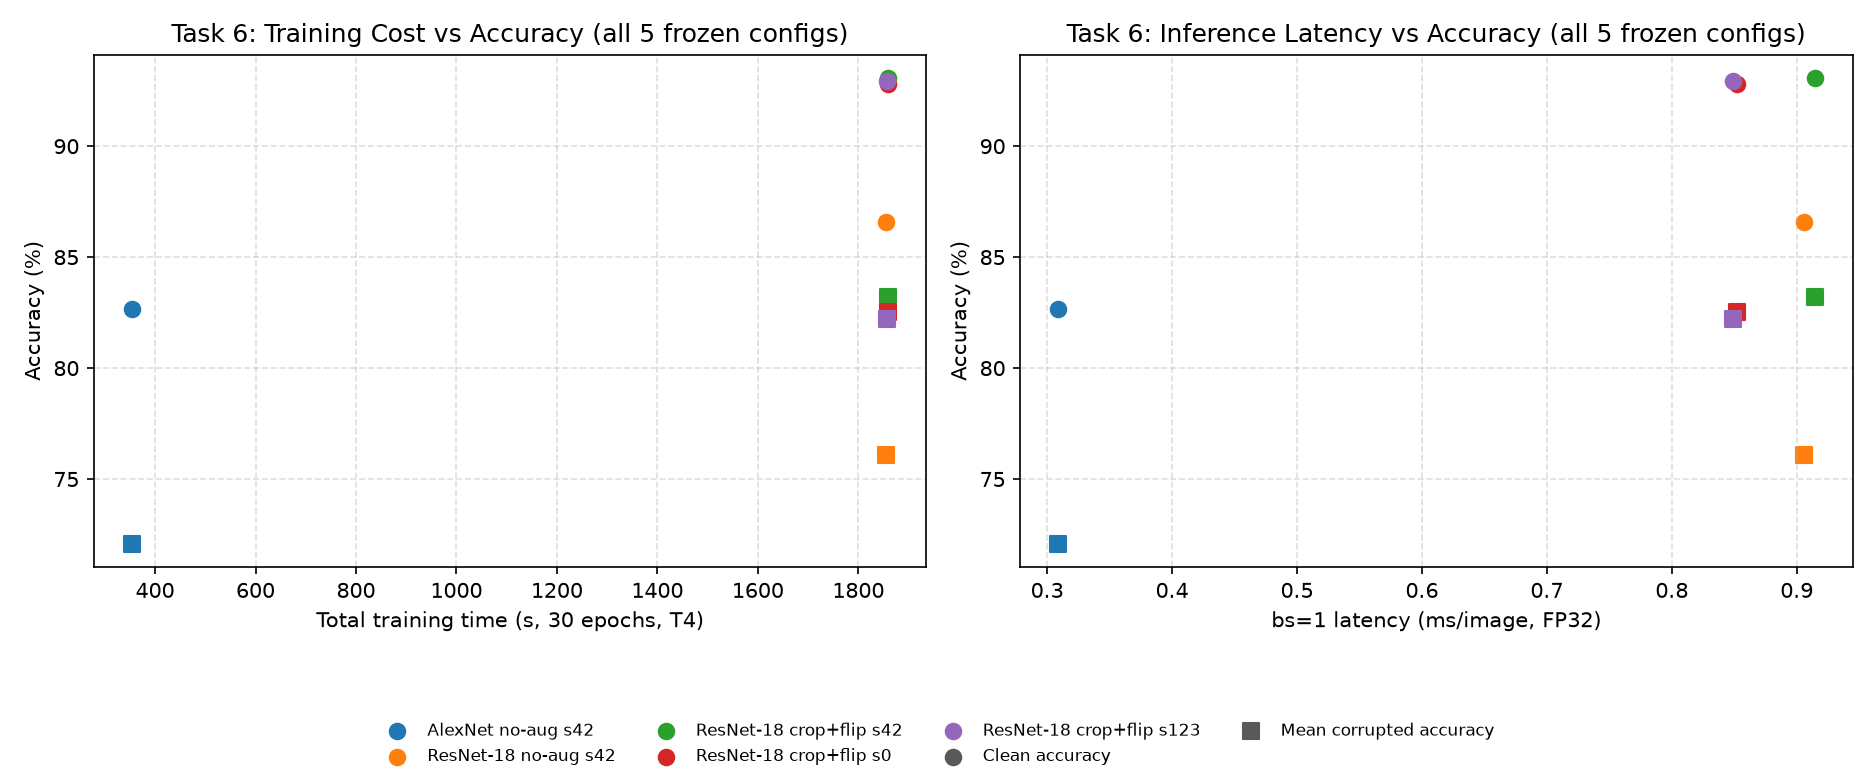
\includegraphics[width=0.95\textwidth]{../results/figures/t6_tradeoffs.png}
\caption{Training time on the T4 and batch-1 latency on the Jade GPU against
clean and mean corrupted accuracy for all five configurations.}
\label{fig:t6-tradeoffs}
\end{figure}

\begin{figure}[H]
\centering
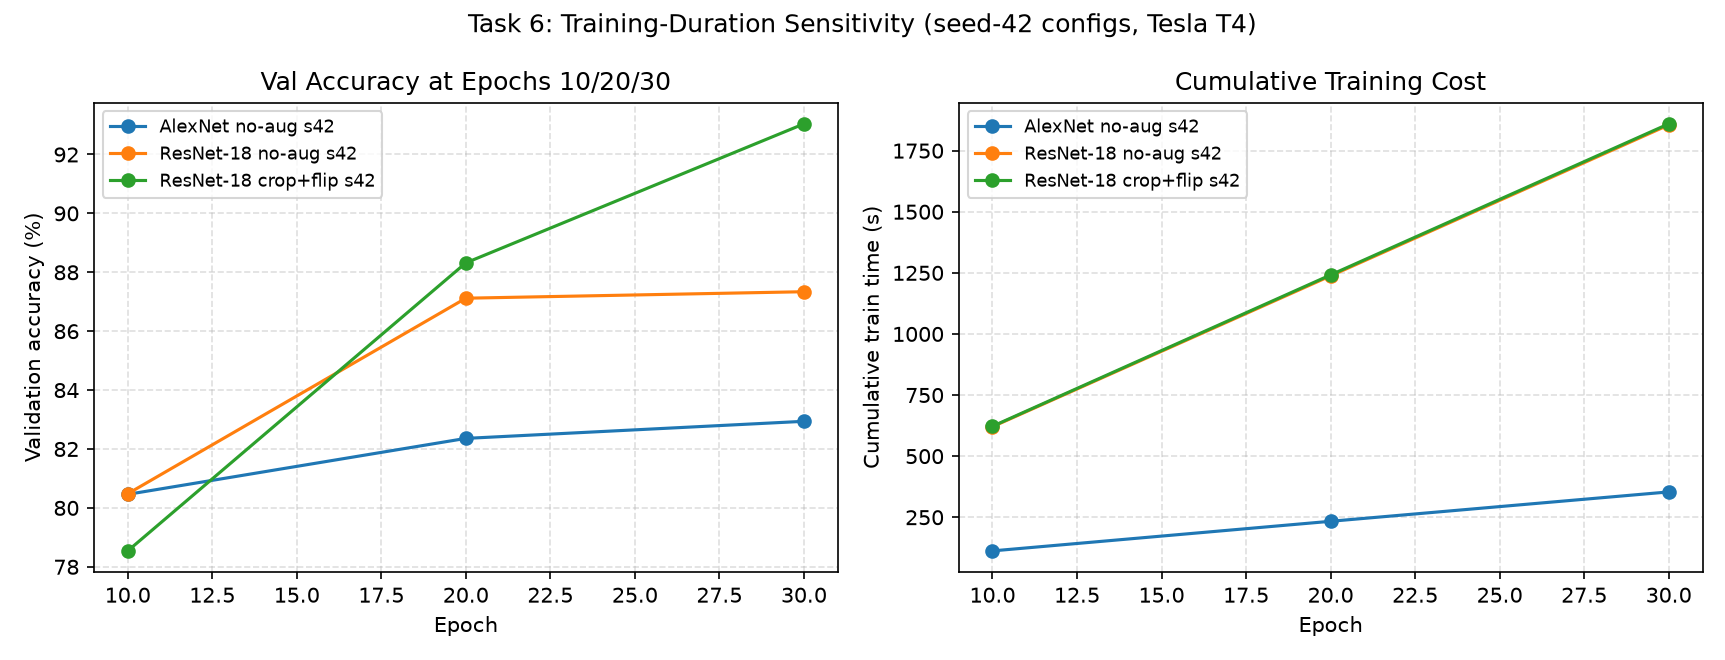
\includegraphics[width=0.95\textwidth]{../results/figures/t6_training_duration.png}
\caption{Validation accuracy at epochs 10, 20, and 30 against cumulative T4
training time for the three seed-42 configurations.}
\label{fig:t6-duration}
\end{figure}

% =====================================================================
\clearpage
\section*{Limitations and next experiment}
\tocentry{Limitations and next experiment}

The no-augmentation versus augmentation comparison rests on a single seed-42
pair, and only the augmented ResNet has three seeds. The corruption suite is
one fixed realization of three mild corruption types, so the robustness
claims do not extend to other corruption families or severities. Training
and inference timing come from different machines and are reported
separately, which rules out direct cross-hardware ranking. Finally, no
augmentation search was performed, so crop plus flip is a reasonable default
rather than a tuned choice.

The clearest measured weakness in the recommended ResNet family is Gaussian
noise: it is the worst condition for all three augmented ResNets (0.6615 to
0.6814, with clean-minus-corrupted drops of 0.2494--0.2677 across seeds 42,
0, and 123), and adding crop plus flip made it worse rather than better. The controlled follow-up experiment keeps
every setting of \texttt{t4\_resnet18\_cifar\_crop\_flip\_s42} fixed (same
architecture, seed 42, 30 epochs, optimizer, schedule, split, and batch
size) and adds training-time Gaussian noise with standard deviation 0.05 to
the crop plus flip pipeline, matching the evaluation distribution. The
existing crop plus flip run serves as the control, so the only changed
variable is noise exposure during training. Re-evaluating on the same frozen
corruption suite and the same STL-10 protocol would test whether training
noise exposure improves noise accuracy while preserving clean and geometric
performance. This experiment has not been run, and no result is claimed for
it.

\section*{Conclusion}
\tocentry{Conclusion}

For the seed-42 ResNet pair, crop plus flip is nearly free on the T4
($+0.24\%$ training time, identical memory) and buys $+0.0650$ clean
accuracy, $+0.1191$ under rotation, and $+0.1267$ under translation. The
augmented model has the smallest CIFAR-to-STL domain drop among the three
seed-42 models (0.1231), which is a frozen generalization observation rather
than a selection criterion. Its Gaussian noise accuracy is 0.6814, compared
with 0.7133 for the no-augmentation ResNet. Across seeds 42, 0, and 123, the
crop-plus-flip ResNet-18 family gives the strongest accuracy-cost balance;
AlexNet is the latency-first alternative at roughly one third of the
batch-1 latency. The main open weakness for the recommended ResNet is noise
robustness, and the single controlled experiment above tests whether adding
noise exposure during training helps without sacrificing clean or geometric
accuracy.

\section*{Reproduction and artifacts}
\tocentry{Reproduction and artifacts}

\begin{itemize}[leftmargin=1.5em]
  \item Executed notebook with all outputs:
    \nolinkurl{lab1/notebooks/role_c_task4_challenge2_task6.ipynb}
  \item Result JSON files (corruption metrics, per-class accuracy,
    Challenge 2 summaries, inference benchmarks):
    \nolinkurl{lab1/results/t4_*.json} and \nolinkurl{lab1/results/t6_*.json}
  \item Summary tables: \nolinkurl{lab1/results/role_c_summary.csv},
    \nolinkurl{lab1/results/task6_seed_sensitivity.csv},
    \nolinkurl{lab1/results/task6_training_duration.csv},
    \nolinkurl{lab1/results/task6_hardware_comparison.csv}; per-epoch
    histories in \nolinkurl{lab1/results/histories/}
  \item Per-image prediction archives:
    \nolinkurl{lab1/results/predictions/<exp_id>.npz} (10,000 shared CIFAR
    IDs per condition, 7,200 STL IDs, identical across the five files)
  \item Figures: \nolinkurl{lab1/results/figures/}
  \item Corruption protocol: \nolinkurl{lab1/configs/corruptions_t4.json};
    implementation in \nolinkurl{lab1/src/corruptions.py} and
    \nolinkurl{lab1/src/run_role_c_experiments.py}
  \item Checkpoints are not in Git; the five \texttt{best.pt} files live in
    Google Drive and in the Jade working directory, as recorded in
    \nolinkurl{lab1/results/checkpoints_manifest.json}
\end{itemize}

\begin{thebibliography}{9}
\bibitem{cifar10}
A.~Krizhevsky.
\newblock Learning Multiple Layers of Features from Tiny Images (CIFAR-10
dataset), 2009.
\newblock \url{https://www.cs.toronto.edu/~kriz/cifar.html}

\bibitem{alexnet}
A.~Krizhevsky, I.~Sutskever, and G.~Hinton.
\newblock ImageNet Classification with Deep Convolutional Neural Networks.
\newblock NeurIPS 2012.

\bibitem{resnet}
K.~He, X.~Zhang, S.~Ren, and J.~Sun.
\newblock Deep Residual Learning for Image Recognition.
\newblock CVPR 2016.

\bibitem{stl10}
A.~Coates, A.~Ng, and H.~Lee.
\newblock An Analysis of Single-Layer Networks in Unsupervised Feature
Learning (STL-10 dataset).
\newblock AISTATS 2011.
\newblock \url{https://cs.stanford.edu/~acoates/stl10/}
\end{thebibliography}

\end{document}
